
\chapter{系统实现 }

\label{chp:implement}

\eat{

RunDroid使用Java作为开发语言,使用了srcML、Xposed、Neo4j等技术,由预处理器、运行时拦截器、日志记录器、调用图构建器等部分组成。
本章将详细的介绍上述技术及RunDroid各组成部分的实现细节。
}



在技术实现上,RunDroid主要分为预处理器、运行时拦截器、日志记录器、调用图构建器等4个部分,对应的工作流程如\autoref{fig:rundroid_overview}所示。
%从功能上,预处理器和运行时拦截器两者的作用是一致的:在程序运行过程中,当相关方法执行时,触发日志记录器记录相应的信息。
预处理器通过源代码插桩技术实现在用户方法运行时触发用户方法的信息记录,而运行时拦截器则是通过方法劫持技术实现对系统方法执行的拦截,进而触发日志记录。
%系统方法的执行。
%由于,用户方法层面的代码已修改,而系统方法的行为难以修改
%并非所有的方法都是进行日志代码织入的。RunDroid可以接触到用户方法(开发者在应用层面定义的方法)的源代码,而对于前者,
在应用运行时,日志记录器会以日志的形式将用户方法和系统方法对应的执行信息记录下来。
最后,调用图构建器会根据应用程序运行时输出的日志,构建拓展函数调用图。

\begin{figure*}[!hb]
	\centering
	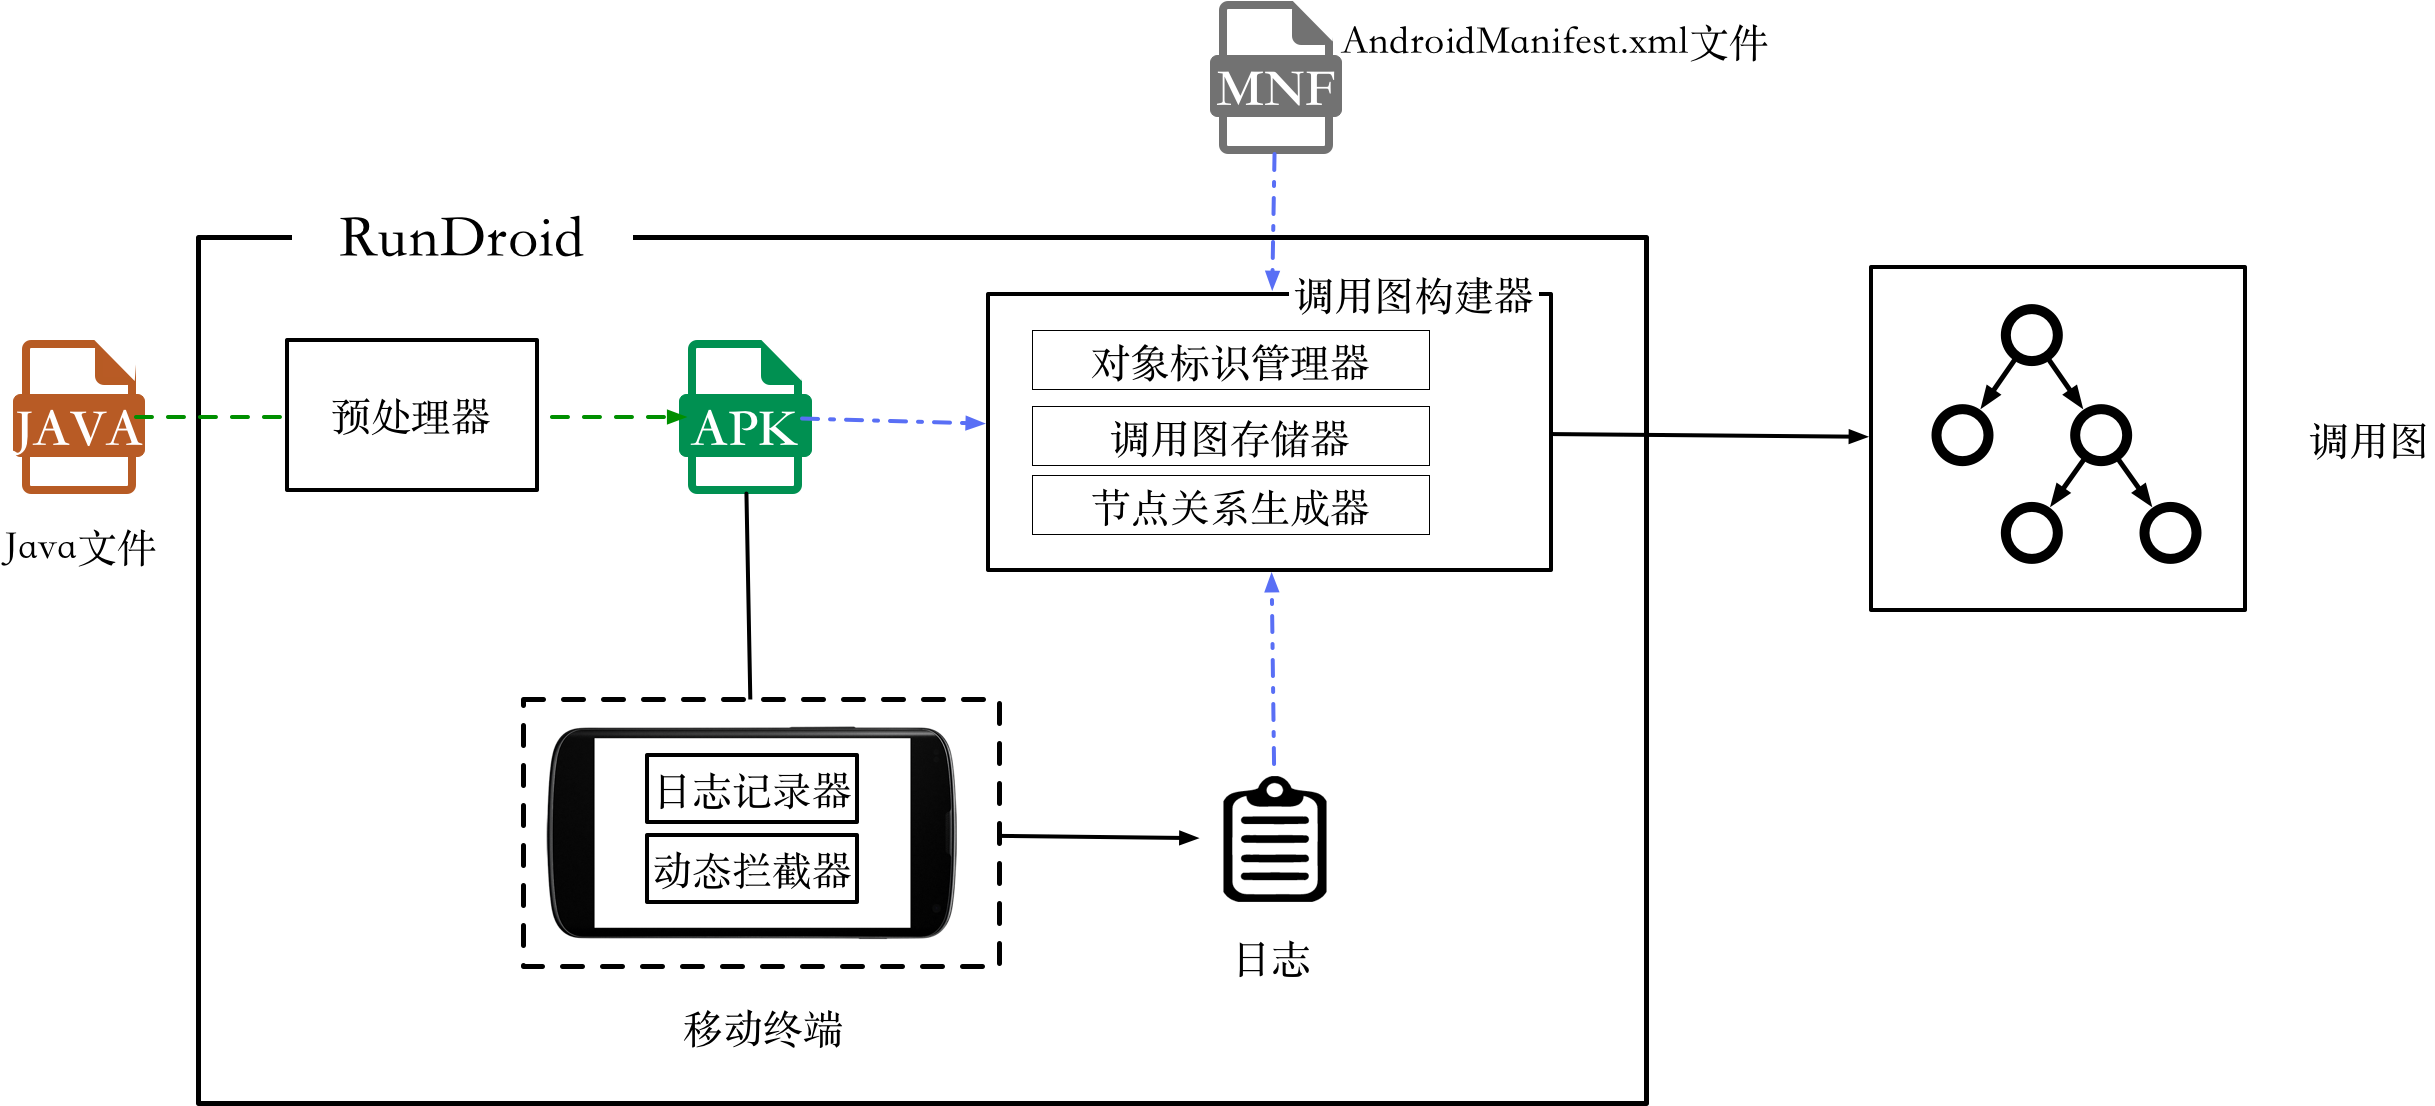
\includegraphics[width=0.8\textwidth]{./Figures/rundroid-overview.png}
	\caption{ RunDroid的工作流程}
	\label{fig:rundroid_overview}
\end{figure*}


\section{模块实现}



\subsection{预处理器}

预处理器在RunDroid中的作用主要是用户方法的日志代码编织。
在现有的技术上,代码编织主要分为两类:基于源代码的代码编织和基于字节码的代码编织。
字节码编织技术以AspectJ\cite{TheAspecJ}为典型代表,技术成熟,应用广泛。
但是,字节码插桩技术在运行过程中会生成过多的方法数,在Android应用构建过程中可能存在方法数65K限制问题。
为此,预处理器采用的方案是基于源代码的代码编织方案。

在实现上,预处理器利用轻量级源代码分析工具srcML\cite{collard2013srcml}对程序的源代码进行语法解析,将程序的抽象语法树转化成XML文件。
在XML文件的基础上,预处理器直接对每个方法体进行修改,实现日志代码的编织,最后重新转换成源代码,经过构建得到可以运行的APK文件。
该方案通过直接修改源程序,将日志记录代码写入在方法体内部,避免了新方法的引入,规避了方法数65K限制问题。

%它可以,支持C、C++、C\#以及Java等多个语言的语法解析。
%	同时,srcML还提供了一个强大工具集,支持对生成内容的查询、分析以及修改,可以用于架构设计、语言研究、软件重构等场景,应用于软件工程、编程语言、并行和分布式处理等多个领域。
%在RunDroid,srcML作为RunDroid预处理器中的重要组成部分,承担源代码语法解析的主要职责,辅助完成用户方法层面的日志代码的编织。
% 拦截器组件基于Xposed框架[5],它拦截在应用程序层和Android框架之间传递的消息。
% 拦截器记录在两个层之间进行的每个方法调用,并将它们与应用程序层中对应的方法调用相关联,以产生完整的方法调用跟踪。
% RunDroid维护感兴趣的方法列表,如生命周期方法和隐式回调,以便日志文件包含每次执行期间调用的方法调用

\subsection{运行时拦截器}%——系统方法的捕获}

%由于预处理器可以处理的方法需要
由于无法对系统方法的源代码进行直接修改,因此预处理器无法实现对系统方法的日志代码编织。
为了弥补预处理器的不足,RunDroid中的运行时拦截器需要在系统层面上实现对系统方法的拦截,实现后续方法信息的日志记录。


%Interceptor组件构建在Xposed框架[5]之上,它拦截在应用程序层和Android框架之间传递的消息。 
%Interceptor记录在两个层之间进行的每个方法调用,并将它们与应用程序层中的相应方法调用相关联,以生成完整的方法调用跟踪。
 %RunDroid维护一组感兴趣的方法,例如生命周期方法和隐式回调,以便日志文件包含每次执行期间调用的方法调用。

%xposed是一个模块框架,可以在不接触任何APKs的情况下改变系统和应用程序的行为。这很棒,因为这意味着模块可以在不做任何改变的情况下为不同版本甚至是rom工作(只要原始代码没有太多改变)。撤销也很容易。由于所有更改都在内存中完成,您只需关闭模块并重新启动即可恢复原始系统。还有许多其他优点,但这里还有一个:多个模块可以对系统或应用程序的同一部分进行更改。有了改进的APKs,你可以选择一个。除非作者用不同的组合构建多个APKs,否则无法将它们组合起来。


%posed是一个基于Android系统的运行时行为修改框架。
%在不修改程序源代码的情况下,基于Xposed开发的第三方插件通过将目标方法关联到函数执行回调上,进行方法参数和返回值的重写和额外方法逻辑的添加等操作,达到目标方法行为修改的目的。
%	Xposed的实现原理具体如下:由于Android系统的所有的应用程序进程都是由Zygote进程孵化而来,Xposed通过替换程序\code{/system/bin/app\_process},使得系统在启动程中加载Xposed的相关文件,将所有的目标方法指向Native方法xposedCallHandler,维护目标方法和对应的钩子方法(Hook Function)的映射关系,从而实现对Zygote进程及Dalvik虚拟机的劫持;
% 当程序执行到目标方法时,xposedCallHandler会完成目标方法的原有代码和对应钩子方法的调度,达到对目标方法劫持的目的。
%利用Xposed提供的类似面向切面编程的API接口,RunDroid中的运行时拦截器可以对任意方法(包括用户方法和系统方法)执行过程进行动态拦截,达到系统方法信息的日志记录的目的。


在实现上,运行时拦截器是基于Xposed\cite{Xposed}实现的插件,它维护的列表包括了所有需要拦截的系统方法(下称为目标方法)。%,如\autoref{tbl:hookMethodList} 所示。
每当目标应用程序启动时,运行时拦截器通过Xposed提供的API\code{ XposedHelpers.findAndHookMethod()}将\autoref{tbl:hookMethodList}中的目标方法绑定到方法钩子(即\eat{Xposed提供的XC\_MethodHook的子类 ,}类HookCallBack)上。
在应用程序的运行过程中,HookCallBack对象的方法\code{beforeHookedMethod(MethodHookParam)}会在目标方法执行之前被调用,
方法\code{afterHookedMethod(MethodHookParam)}会在目标方法执行后调用。
上述两个方法的参数\code{MethodHookParam}中会包括该方法执行时的相关方法对象。
最终,HookCallBack对应会将方法执行的相关信息传递给日志记录器。



相比定制化Android系统,通过Xposed实现的运行时拦截器兼容性良好,适用于市面上主流的Android系统版本,实现成本低。
同时,待拦截方法列表的编辑功能的引入,使得在不修改插件代码的情况下,支持动态添加删除待拦截的方法,避免了Xposed插件修改后的系统重启操作,提高了RunDroid整体的运行效率。
 

\subsection{日志记录器}

日志记录器的职责是将方法执行的消息以日志文件的形式进行持久化存储。
针对不同的方法类型(静态方法与非静态方法、用户方法与系统方法等),日志记录器提供了不同的API,帮助我们记录相应方法执行的日志信息。
在日志内容上,日志记录器还会记录每个方法执行的时间戳、所处线程、方法签名标识、所处阶段(方法开始执行阶段/方法执行完毕阶段)以及相关的方法对象信息。
方法对象信息主要包括对象的类型、属性和全局ID(通过Java API\code{System.identityHashCode(Object)}获取)等。
同时,日志记录器还支持对象信息的自定义:开发人员可以根据自身的需要为不同类型的对象输出不同对象数据信息。
% 在底层实现上,考虑日志读入文件对程序执行效率的影响,我们评估了多种日志写入方式,最终我们发现基于mmap的日志记录方式效率最高,对程序运行的影响最小。




\subsection{调用图构建器}

% 调用图构建器的功能是拓展函数调用图的构建、存储和展现。
调用图构建器由调用图存储器、对象管理器和关系生成器组成,如\autoref{fig:rundroid_overview}所示。

调用图存储器将Neo4j\cite{Neo4jthe19}作为调用图的底层存储引擎,承担着拓展函数调用图的存储、查询、展示的职责。
Neo4j的数据分为节点(Node)和关系(Relationship)两大类型,支持自定义键值属性。
同时,Neo4j可为节点指定标签,为关系指定类型,用于区分不同含义的节点和关系。
拓展函数调用图中的数据在Neo4j中的表现形式如下:
调用图中的方法和对象会以节点的形式出现在调用图中, 方法节点的标签分为\code{METHOD}和\code{FRAMEWORK},对象节点的标签为\code{OBJECT};
方法和方法的关系分为调用关系和触发关系,在Neo4j中分别用关系\code{INVOKE}和\code{TRIGGER}表示;
方法和对象之间的关系分为参数关系、返回值关系和实例关系,在Neo4j中分别用关系\code{PARAMETER}、\code{RETURN}、\code{INSTANCE}表示。




\eat{
	Neo4j是基于Java语言开发的图数据库,可以用于存储图结构相关的数据结构。
	%与传统的基于关系模型的存储结构不同,Neo4j的存储模型是基于图论开发的,遵循属性图数据模型。


	在数据操作接口方面,Neo4j支持Cypher、Java API和RESTful API等方式,提供友好的数据浏览界面用于数据的展示与修改。
	\eat{由于基于属性图数据模型,Neo4j通常适用于和图关系有着密切关系的应用场景:例如社交网络分析,公共交通网络研究以及地图网络拓扑等场景。}
	在RunDroid,Neo4j是调用图构建器的主要组成部分,承担着拓展函数调用图的存储、查询、展示的职责。
}


对象管理器负责将日志中的对象信息映射成调用图中的节点。
通常情况下,我们认为对象和全局ID一一对应,所以,我们将全局ID相同的对象信息映射成调用图中的一个节点。
但考虑到有些类型(例如Handler机制中的Message)使用对象池技术,我们还在全局ID的基础上引入对象版本号,避免对象在不同生命周期的串用。
以Message为例,调用图构建过程中,如果对象管理器发现待提交的Message对象$m$是方法\code{Message.obtain()}的返回值,处理逻辑如下:
如果调用图中不存在一个全局ID和$m$一致的节点,则对象管理器会创建一个全新的节点来表示$m$,设置其对象版本号为1;
而调用图已经存在一个全局ID和$m$一致,版本号为$version$的节点$m'$,则对象管理器会创建一个全新的节点来表示$m$,并将$version + 1$作为节点$m$的版本号,而不是复用原有节点象$m'$。
因此,在对象管理器的角度看来,两个Message对象只有当全局ID和对象版本号都一致时,才是同一个对象。



关系生成器是第\ref{chp:design}章中\autoref{alg:buildCG}、\autoref{alg:buildActivityLifecycle}、\autoref{alg:buildTrigger}的具体实现,基于Cypher脚本和Soot完成。
例如,\autoref{alg:buildTrigger}第16$\sim$17行中,我们需要找到使用$o_{m}$作为参数的方法$m_{enqueue}$、$m_{dispatch}$,并建立两者之间的触发关系。
传统的实现方式需要对图进行遍历,效率较低。而RunDroid采用了Cypher脚本,实现简洁,开发效率高,如\autoref{fig:cypher_code}所示。
Soot的工作主要是提供应用程序相关的类型查询服务。
例如,\autoref{alg:buildTrigger}第7行中,我们需要知道所有的Runnable对象,此处便需要通过Soot查询所有的Runnable子类。
另外,在算法\ref{alg:buildActivityLifecycle}中,我们也会将Soot和Cypher相结合用于查找所有Activity的生命周期方法。


\begin{figure}[!h]
	\centering
	%normal
	\begin{lstlisting}[style=normal,language=cypher]
	MATCH (m_enqueue:METHOD)-[:PARAM]->(o_m:OBJECT),
					(m_dispatch:METHOD)-[:PARAM]->(o_m:OBJECT)
	return o_m, m_enqueue, m_dispatch\end{lstlisting}
	\caption{使用Cypher查找共用对象$o_m$的方法$m_{enqueue}$、$m_{dispatch}$}
	\label{fig:cypher_code}
\end{figure}


 \section{本章总结}

本章侧重介绍RunDroid的系统实现。
在整体上,RunDroid由预处理器、运行时拦截器、日志记录器、调用图构建器等部分组成。
预处理器和运行时拦截器分别对应应用程序在执行过程中用户方法和系统方法的执行拦截,以触发日志记录器记录方法执行信息。
预处理器是通过源代码编织实现的,避免了新方法的引入,规避了方法数65K限制问题。
运行时拦截器借助Xposed框架提供的方法执行劫持技术实现对系统方法的执行拦截,在实现上规避了Xposed插件修改后的重启系统操作。
调用图构建器将运行过程中方法执行的日志信息作为输入,在Neo4j图数据库上构建函数调用图,利用图中方法和对象之间的关系,利用Soot和Cypher语句实现Activity生命周期的构建、方法触发关系的生成。
